\section{2.1-2.3}
\subsection{Agents and environnements}
	\begin{figure}[H]
		\centering
		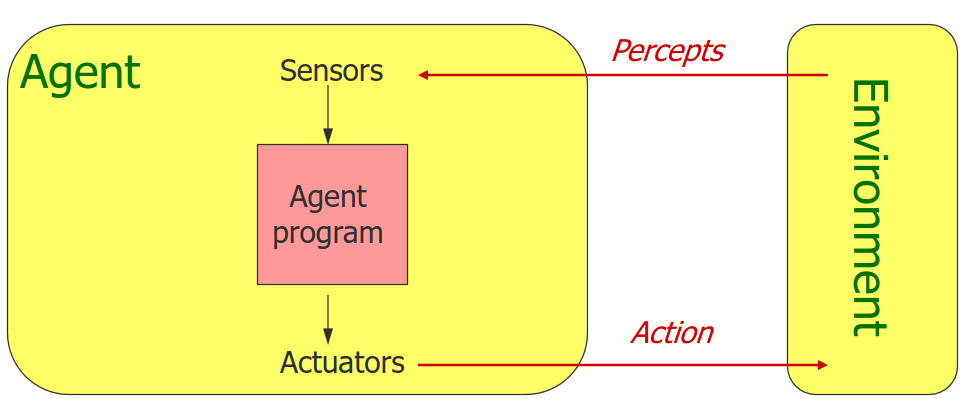
\includegraphics[width=\textwidth]{img/agent.png}
		\caption{Agent}
	\end{figure}
	
	\begin{itemize}
		\item \textbf{Agent} : Entité qui interagi avec son environnement, perception avec des sensors et action avec des actuators
		\item \textbf{Percept} : Perception de l'agent a un instant $t$
		\item \textbf{Percept sequence} : Historique complet des percept d'un agent
	\end{itemize}
\subsection{Concept of Rationality}

	\textbf{Rationalité} : " Faire la bonne action ", l'action qui amène au meilleur résultat. Mais un ordinateur ne sais pas c'est quoi la bonne chose a faire. On va donc avoir besoin d'une \textbf{Performance measure} qui va calculer un score si l'action est bonne ou pas.
	
	\textbf{Agent rationnel} : Pour chaque séquence d'action possible, un agent rationnel doit sélectionner un action qui maximise la \textbf{Performance measure}.
	
	La rationalité d'un action dépend de :
	\begin{enumerate}
		\item Une \textbf{Performance measure} qui dépend des critères de succès
		\item La connaissance préalable de l'environnement par l'agent
		\item Les actions que l'agent peut faire
		\item La séquence de perception actuelle de l'agent
		
	\end{enumerate}
	
	Attention, \textbf{Rationality $\neq$ Omniscience}
	
	\textbf{Agent omniscient} : sait le réel résultat de ses actions
	
	\textbf{Agent autonome} : apprend ce qu'il peut faire pour compenser ce qu'il ne sait pas faire. (machine learning)
	
\subsection{Nature et environnements}
	Environnement de travail d'un agent est spécifique a (PEAS) \textbf{P}erformance, \textbf{E}vironnement, \textbf{A}ctuators, \textbf{S}ensors.
	
	\begin{figure}[H]
		\centering
		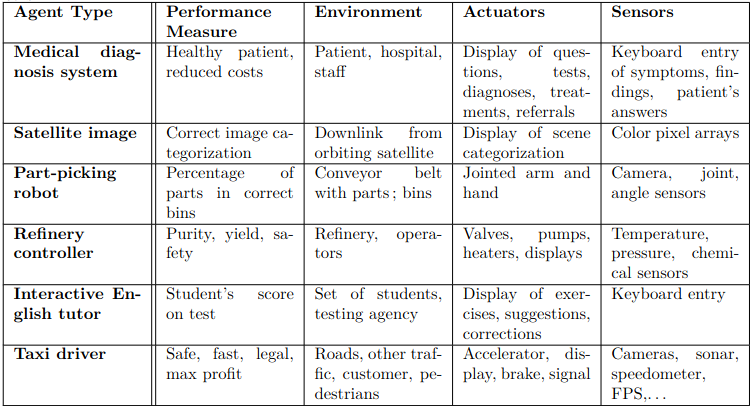
\includegraphics[width=\textwidth]{img/PEASexemple.png}
		\caption{Exemple PEAS}
	\end{figure}	
	
	Les propriété sont les suivante:
	
	\textbf{Fully observable vs. Partially observable} : Toutes les informations pertinentes sont accessibles (échecs vs poker)
	
	\textbf{Single agent vs. Multiagent} : il y a t'il plus que 1 agent, si oui c'est une compétition ou coopération ? (crossword puzzle vs chess)
	
	\textbf{Deterministic vs. Stochastic} : (Chess vs.Poker)
	\begin{itemize}
		\item Le prochain état (state) de l'environnement dépend entièrement de l'action de l'agent.
		\item L'environnement pour l'agent est moins déterministe car il ne dispose pas de toutes les informations sur l'environnement.(Il ne peut pas déterminer avec précision l'état suivant à cause du hasard).
	\end{itemize}
	\textbf{Episodic vs. Sequential} : L'expérience de l'agent est divisée en épisodes atomiques indépendants les uns des autres.
	
	\textbf{Static vs. Dynamic} : L'environnement peut changer quand l'agent est entrain de réfléchir.
	
	\textbf{Discrete vs. Continuous} : Le nombre différent de state est fini et l'ensemble des actions est discret (chess vs. taxi driving)
	
	\textbf{Known vs. Unknown} : le résultat de chaque action est donné. Ce n'est pas la même chose que d'être totalement observable, par exemple les jeux vidéo, on connaît toutes les informations via l'écran mais on ne sait pas ce que fait le bouton.
	
	\begin{figure}[H]
		\centering
		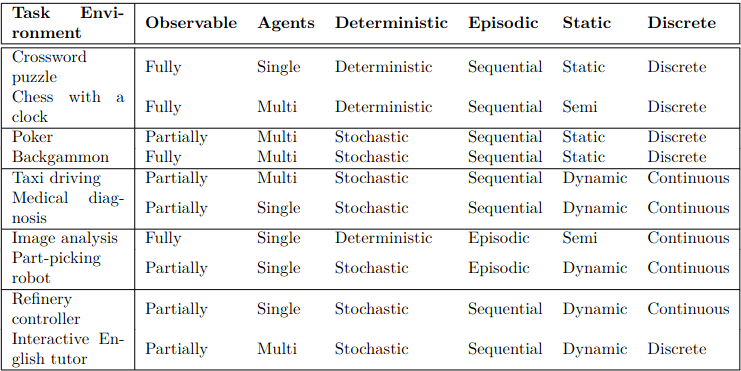
\includegraphics[width=\textwidth]{img/PEASexemple2.png}
	\end{figure}